\chapter{STUDI LITERATUR}

Bab ini memberikan pengetahuan prasyarat yang mendasari isi dari tugas akhir ini. Secara spesifik, bab ini membahas dasar teori probabilitas yang digunakan, aplikasinya dalam estimasi keadaan probabilistik, dan algoritma terkait; struktur dan cara kerja modul terkait pada perangkat lunak robot sepak bola tim Dagozilla; dan studi terkait yang sudah ada pada topik estimasi keadaan multiagen maupun estimasi keadaan dengan latensi data.

\section{Teori Probabilitas}

\subsection{Teorema Bayes}
Analog dengan definisi yang ada pada probabilitas kejadian, didefinisikan juga peluang kondisional
\begin{align}
    p(x \,|\, y) = Pr(X = x \,|\, Y = y) = \frac{p(x, y)}{p(y)}
\end{align}
yang digunakan untuk memodelkan peluang nilai $x$ terjadi apabila nilai $y$ terjadi. Dua variabel acak $X$ dan $Y$ disebut independen apabila untuk semua kemungkinan $x$ dan $y$ berlaku
\begin{align}
    p(x, y) = p(x) p(y) \quad\textit{atau}\quad p(x \,|\, y) = p(x)
\end{align}

Terkait peluang kondisional, Teorema Bayes menyatakan bahwa
\begin{align}
    p(x \,|\, y) = \frac{p(y \,|\, x)\, p(x)}{p(y)} = \eta\, p(y \,|\, x)\, p(x)
\end{align}
dimana $\eta = p(y)^{-1}$ merupakan suatu nilai yang konstan untuk semua kemungkinan $x$. Karena jumlah dari semua nilai $p(x \,|\, y)$ haruslah bernilai satu, $\eta$ disebut juga faktor normalisasi dan dapat ditentukan kemudian sebagai jumlah dari nilai $p(y \,|\, x)\, p(x)$ untuk semua kemungkinan $x$.

Teorema Bayes sangat berguna untuk memperbarui kepercayaan terhadap distribusi peluang $x$ setelah mengetahui terjadinya $y$ apabila diketahui peluang terjadinya $y$ dapat ditentukan untuk setiap kemungkinan $x$.

\subsection{Distribusi Gaussian}

Salah satu distribusi yang penting dan banyak dipelajari adalah keluarga distribusi Gaussian atau distribusi normal dimana dengan nilai rata-rata $\mu$ dan nilai variansi $\sigma^2$ memiliki fungsi densitas
\begin{align}
    p(x) = \frac{1}{\sigma \sqrt{2\pi}} \exp\left\{-\frac{1}{2}\left(\frac{x-\mu}{\sigma}\right)^2\right\}
\end{align}
dengan kasus spesial dimana $\mu = 0$ dan $\sigma^2 = 1$ disebut juga distribusi normal standar.

Distribusi Gaussian banyak dipelajari karena beberapa alasan. Salah satu alasan adalah karena distribusi ini memiliki banyak properti yang membuatnya mudah dimanipulasi dan digunakan, diantaranya adalah fungsi distribusi penjumlahan variabel-variabel acak independen berdistribusi Gaussian, maupun perkalian dan konvolusi fungsi Gaussian juga merupakan fungsi Gaussian. Alasan lainnya adalah diobservasi juga berbagai variabel acak di berbagai pengujian ilmiah yang ternyata memiliki distribusi yang hampir mirip dengan Gaussian. Selain itu juga, terbukti bahwa berdasarkan Teorema Limit Pusat, rata-rata dari banyak variabel acak distribusi identik independen akan mendekati distribusi Gaussian. (\cite{degroot2012})

Disebabkan oleh alasan-alasan tersebut, praktisnya distibusi Gaussian banyak digunakan untuk memodelkan berbagai variabel acak di dunia nyata, seperti distribusi sampel dari populasi yang sangat besar maupun distribusi error pada suatu pengukuran atau kontrol sering diasumsikan memiliki distribusi Gaussian.

Distribusi Gaussian memiliki generalisasi ke dalam vektor acak yaitu kumpulan variabel acak yang direpresentasikan dalam bentuk vektor. Dengan parameter vektor rata-rata $\mu$ dan matriks kovarian $\Sigma$ yang bersifat simetrik dan positif semidefinit, didefinisikan fungsi densitas
\begin{align}
    p(x) = det(2 \pi \Sigma)^{-\frac{1}{2}} \exp\left\{-\frac{1}{2}(x-\mu)^T \Sigma^{-1} (x-\mu)\right\}
\end{align}
dimana masing-masing komponen $X_i$ sendiri memiliki distribusi Gaussian dengan rata-rata $\mu_i$ dan kovarian antara $X_i, X_j$ sama dengan $\Sigma_{i,j}$.

\section{Estimasi Keadaan Probabilistik}

Perangkat lunak di robot atau sistem lainnya yang membaca \textit{world state} nyata menggunakan sensor, dan mungkin berinteraksi dengannya menggunakan aktuator, mempunyai kebutuhan untuk menentukan keadaan tersebut dari bacaan sensor. Secara umum, digunakan model matematika yang bertujuan untuk mentranslasi data pengukuran menjadi model \textit{world state}. Seiring berjalannya waktu, penggunaan estimasi \textit{world state} menggunakan model probabilistik menjadi lebih populer dibandingkan model perhitungan yang deterministik. Dengan memodelkan \textit{world state} yang diketahui menjadi suatu distribusi peluang, hasil pengukuran \textit{world state} menjadi lebih tahan terhadap efek error pada data pengukuran. (\cite{thrun2010})

\subsection{Pemodelan Keadaan}

Dalam model probabilistik, \textit{world state} disimbolkan sebagai suatu vektor acak $X$, dimana $x_t$ menandakan \textit{world state} pada waktu ke-$t$. Vektor acak ini mengandung berbagai variabel acak misalnya posisi dan orientasi sesungguhnya dari robot maupun objek lain pada suatu waktu.

Sistem melakukan pengukuran terhadap dunia yang disimbolkan sebagai vektor acak $Z$ dan instansiasinya $z_t$ yang merupakan pengukuran dari dunia nyata pada waktu ke-$t$. Sedangkan apabila sistem melakukan interaksi umpan balik terhadap dunia nyata menggunakan suatu aktuator yang dikontrol oleh sistem, maka perintah interaksi tersebut disimbolkan sebagai vektor acak $U$ dan $u_t$ yang merupakan kontrol interaksi saat sistem sedang melakukan transisi dari $x_{t-1}$ ke $x_t$.

Perhatian dari estimasi keadaan probabilistik adalah mengestimasi nilai dari $x_t$ diberikan nilai $z$ dan $u$ yang terjadi sebelumnya. Dalam persamaan matematika, hendak dihitung
\begin{align}
    bel(x_t) = p(x_t \,|\, z_{1:t}, u_{1:t}) \,,
\end{align}
atau distribusi peluang alternatif dimana diprediksi nilai dari $x_t$ sebelum mendapat hasil pengukurannya $z_t$,
\begin{align}
    \overline{bel}(x_t) = p(x_t \,|\, z_{1:t-1}, u_{1:t}) \,.
\end{align}

Mengasumsikan nilai $X$ mengandung semua \textit{world state} yang relevan terhadap sistem pada waktu sekarang, maka tidak ada informasi tambahan yang bisa diberikan oleh pengukuran $z_t$ maupun keadaan sebelumnya $x_{t-k}$ terhadap keadaan berikutnya $x_{t+1}$ di luar apa yang terkandung pada $x_t$. Oleh karena itu dalam pembangkitan nilai $x_t$ dan $z_t$, dua distribusi peluang yang penting diperhatikan adalah peluang transisi keadaan
\begin{align}
    p(x_t \,|\, x_{0:t-1}, z_{1:t-1}, u_{1:t}) = p(x_t \,|\, x_{t-1}, u_t)
\end{align}
dan peluang pengukuran
\begin{align}
    p(z_t \,|\, x_{0:t}, z_{1:t-1}, u_{1:t}) = p(z_t \,|\, x_t)
\end{align}

\begin{figure}[h]
    \centering
    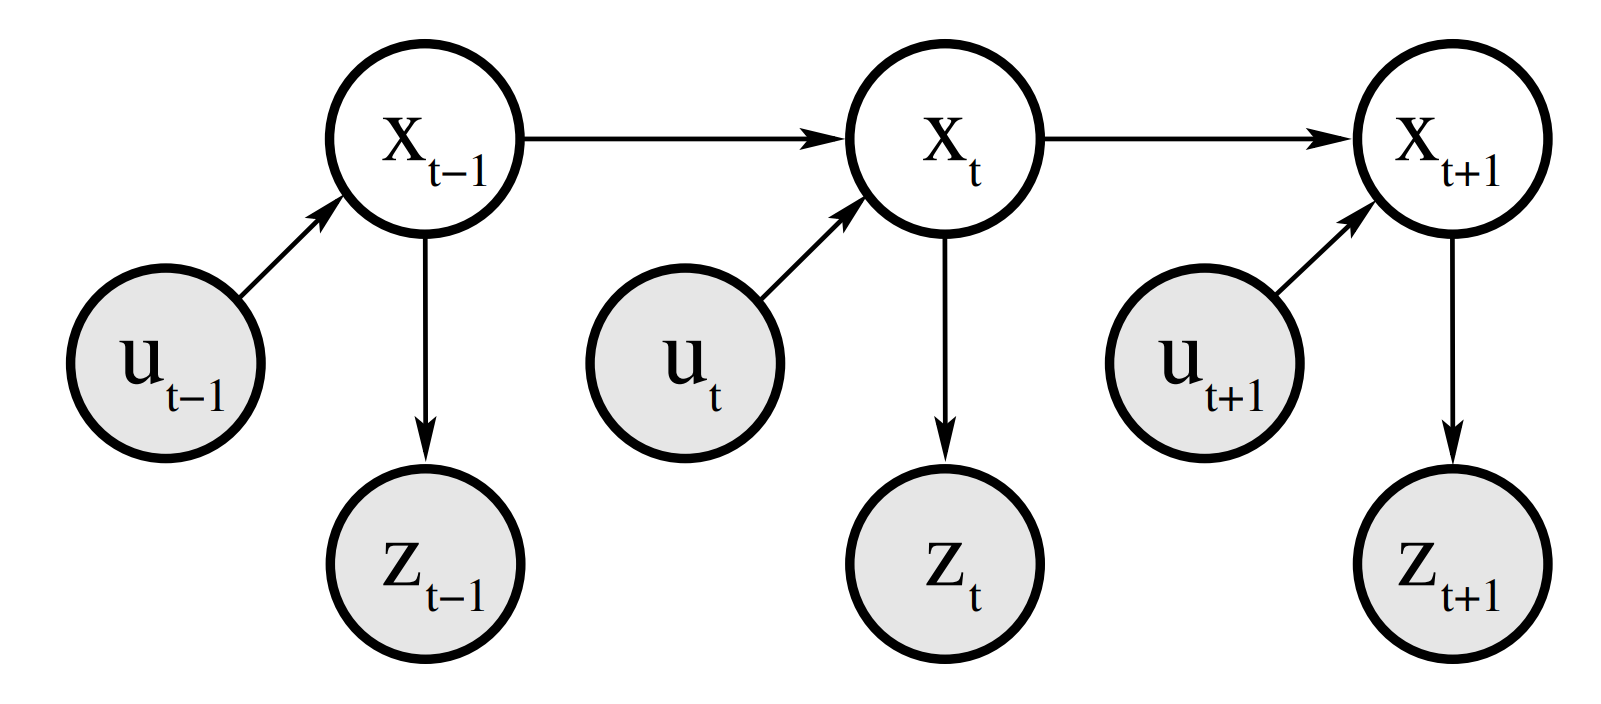
\includegraphics[width=0.8\textwidth]{resources/hidden-markov-model.png}
    \caption{Hubungan $X, U, Z$}
    \label{fig:hidden-markov-model}
\end{figure}

Hubungan ini digambarkan pada gambar \ref{fig:hidden-markov-model}. Peluang yang hanya saling berpengaruh antar tahapan waktu yang berdekatan disebut juga \textit{hidden Markov model} atau \textit{dynamic Bayes network}.

\subsection{Penapis Bayes}

\begin{algorithm}
    \caption{Penapis Bayes}
    \label{alg:bayes-filter}
    \begin{algorithmic}[1]
        \Function{bayes\_filter}{$bel(x_{t-1}), u_t, z_t$}
        \ForAll{$x_t$}
        \State $\overline{bel}(x_t) = \int p(x_t \,|\, u_t, x_{t-1})\, bel(x_{t-1})\, dx_{t-1}$
        \State $bel(x_t) = \eta\, p(z_t \,|\, x_t)\, \overline{bel}(x_t)$ \Comment{$\eta$ menormalisasi nilai dari $bel(x_t)$}
        \EndFor
        \State \Return $bel(x_t)$
        \EndFunction
    \end{algorithmic}
\end{algorithm}

Perhatikan bahwa perubahan nilai dari $\overline{bel}(x_{t-1})$ ke $bel(x_t)$ dapat ditentukan dari peluang transisi keadaan $p(x_t \,|\, x_{t-1}, u_t)$, dan perubahan nilai dari $bel(x_t)$ ke $\overline{bel}(x_t)$ dapat ditentukan dari peluang pengukuran $p(z_t \,|\, x_t)$ menggunakan Teorema Bayes. Memanfaatkan fakta tersebut, dirumuskan algoritma penapis Bayes atau \textit{Bayes filter algorithm} pada algoritma \ref{alg:bayes-filter}. Baris tiga menunjukkan perhitungan nilai $bel(x_t)$ sebagai ekspansi dari penjumlahan nilai $p(x_t, x_{t-1})$ saat diketahui $u_t$ untuk semua kemungkinan $x_{t-1}$, spesifik untuk kasus kontinu. Tahap ini sering disebut tahap prediksi. Baris empat memanfaatkan teorema Bayes untuk mendapatkan distribusi $x_t$ setelah mendapatkan informasi dari $z_t$. Tahap ini sering disebut tahap pembaruan pengukuran.

Algoritma penapis digunakan untuk mengiterasi nilai dari $bel(x_t)$ seiring waktu, dan merupakan algoritma yang optimal mengasumsikan proses merupakan \textit{hidden Markov model}. Perhatikan bahwa algoritma ini mengharuskan pemodelan sendiri nilai dari peluang transisi keadaan, peluang pengukuran, dan distribusi awal $bel(x_0)$ yang akan digunakan.

Selain itu, karena nilai dari $bel(x_t)$ merupakan distribusi peluang, dalam aplikasinya dibutuhkan pendekatan untuk memodelkan distribusi tersebut sehingga dapat dikomputasi oleh komputer. Pada praktisnya, distribusi peluang $bel(x_t)$ dimodelkan sebagai distribusi dengan jenis yang dapat diparameterasikan seperti pada penapis Kalman, atau distribusi tersebut didiskritkan seperti pada penapis histogram atau penapis partikel.

\subsection{Penapis Kalman}

Pada penapis Kalman atau \textit{Kalman Filter} (\textit{KF}), distribusi dari $bel(x_t)$ dan $\overline{bel}(x_t)$ diasumsikan memiliki distribusi Gaussian dengan parameter $\mu$ dan $\sigma^2$ yang dicari pada setiap iterasi algoritmanya. Agar penapis Bayes Gaussian bekerja, distribusi peluang transisi keadaan dan peluang pengukuran harus memiliki restriksi tambahan.

Pada variasi penapis Kalman yang paling sederhana, direstriksi bahwa (1) vektor acak $x_t$ merupakan kombinasi linear dari $x_{t-1}, u_t,$ dan faktor error $\epsilon_t$
\begin{align}
    x_t = A_t x_{t-1} + B_t u_t + \epsilon_t \,
\end{align}
untuk $x_t$ berdimensi $n$, $u_t$ berdimensi $m$, $A_t$ matriks berdimensi $n \times n$, dan $B_t$ berdimensi $n \times m$, dan $\epsilon_t$ vektor acak Gaussian dengan rata-rata nol dan kovariansi $R_t$; (2) $z_t$ merupakan kombinasi linear dari $x_t$ dan faktor error $\delta_t$
\begin{align}
    z_t = C_t x_t + \delta_t
\end{align}
untuk $z_t$ berdimensi $k$, $C_t$ berdimensi $k \times n$, dan $\delta_t$ vektor acak Gaussian dengan rata-rata nol dan kovariansi $Q_t$; dan (3) distribusi awal $bel(x_0)$ memiliki distribusi Gaussian. Ketiga asumsi ini menjamin bahwa distribusi $bel(x_t)$ merupakan distribusi Gaussian untuk semua waktu $t$ yang akan datang.

\begin{algorithm}
    \caption{Penapis Kalman}
    \label{alg:kalman-filter}
    \begin{algorithmic}[1]
        \Function{kalman\_filter}{$\mu_{t-1}, \Sigma_{t-1}, u_t, z_t$}
        \State $\overline{\mu}_t = A_t\, \mu_{t-1} + B_t\, u_t$
        \State $\overline{\Sigma}_t = A_t\, \Sigma_{t-1}\, A_t^T + R_t$
        \State $K_t = \overline{\Sigma}_t\, C_t^T\, (C_t\, \overline{\Sigma}_t\, C_t^T + Q_t)^{-1}$
        \State $\mu_t = \overline{\mu}_t + K_t(z_t - C_t\, \overline{\mu}_t)$
        \State $\Sigma_t = (I - K_t\, C_t)\, \overline{\Sigma}_t$
        \State \Return $\mu_t, \Sigma_t$
        \EndFunction
    \end{algorithmic}
\end{algorithm}

Berdasarkan hubungan di atas, algoritma penapis Kalman menghitung nilai dari parameter rata-rata $\mu_t$ dan kovariansi $\Sigma_t$ dari distribusi Gaussian $bel(x_t)$. Sehingga dapat diturunkan algoritma penapis Kalman seperti pada algoritma \ref{alg:kalman-filter}.

Disebabkan restriksi linearitas pada peluang transisi keadaan dan peluang pengukuran, algoritma penapis Kalman tidak dapat digunakan apabila restriksi linearitas tersebut tidak dipenuhi. Agar penapis Kalman dapat digunakan untuk kasus $x_t = g(u_t, x_{t-1}) + \epsilon_t$ dan $z_t = h(x_t) + \sigma_t$ dimana fungsi $g$ dan $h$ tidak linear, fungsi tersebut harus diaproksimasi terlebih dahulu agar menjadi linear.

Pada \textit{Extended Kalman Filter}, fungsi dilinearkan menggunakan turunan parsial dari fungsi $g$ dan $h$. Dengan menghitung $G_t = g'(u_t, \mu_{t-1})$ dan $H_t = h'(\overline{\mu}_t)$ dimana $g'$ merupakan turunan parsial $g$ terhadap $x_{t-1}$, didapatkan persamaan linear
\begin{align}
    g(u_t, x_{t-1}) \approx g(u_t, \mu_{t-1}) + G_t\, (x_{t-1} - \mu_{t-1}) \\
    h(x_t) \approx h(\overline{\mu}_t) + H_t\, (x_t - \overline{\mu}_t)
\end{align}
Nilai $A$ dan $C$ pada penapis Kalman dapat digantikan dengan nilai $G$ dan $H$.

Pada \textit{Unscented Kalman Filter}, fungsi dilinearkan dengan mengambil sampel nilai pada fungsi $g$ dan $h$, lalu membuat persamaan linear dengan melakukan regresi pada nilai masukan secara umum. Sampel diambil di rata-rata $\mu$ dan dua titik di sekelilingnya untuk setiap dimensi yang ada.

\subsection{Penapis Histogram}

\begin{algorithm}
    \caption{Penapis Bayes Diskrit}
    \label{alg:discrete-bayes-filter}
    \begin{algorithmic}[1]
        \Function{discrete\_bayes\_filter}{$\{p_{k, t-1}\}, u_t, z_t$}
        \ForAll{$k$}
        \State $\overline{p}_{k, t} = \sum_i p(X_t = x_k \,|\, u_t, X_{t-1} = x_i)\, p_{i, t-1}$
        \State $p_{k, t} = \eta\, p(z_t \,|\, X_t = x_k)\, \overline{p}_{k, t}$ \Comment{dinormalisasi untuk semua $k$}
        \EndFor
        \State \Return $\{p_{k, t}\}$
        \EndFunction
    \end{algorithmic}
\end{algorithm}

Pada penapis histogram, kemungkinan nilai dari $x_t$ terbatas dan dibagi-bagi menjadi sebanyak terbatas daerah, misalnya kemungkinan posisi dari robot pada lapangan berdimensi $9 \times 6$ meter persegi dapat dibagi menjadi $1350$ daerah berbentuk persegi berukuran $20 \times 20$ sentimeter persegi dalam suatu grid. Pada algoritma ini, $bel(x_t)$ direpresentasikan sebagai suatu tabel yang menyimpan peluang nilai berada dalam masing-masing daerah yang ada. Algoritma ini pun relatif lebih sederhana karena hanya perlu mendiskritkan perhitungan pada filter Bayes.

Algoritma filter Bayes diskrit ada di algoritma \ref{alg:discrete-bayes-filter}. Apabila fungsi peluang transisi keadaan atau peluang pengukuran yang dimiliki bersifat kontinu, dapat diaproksimasi menjadi diskrit seperti
\begin{align}
    p(\mathbf{x}_{k, t} \,|\, u_t, \mathbf{x}_{i, t-1}) \approx |\mathbf{x}_{k, t}|\, p(\hat{x}_{k, t} \,|\, u_t, \hat{x}_{i, t-1}) \\
    p(z_t \,|\, \mathbf{x}_{k, t}) \approx p(z_t \,|\, \hat{x}_{k, t})
\end{align}
dimana $\hat{x}_{k, t}$ adalah representasi dari daerah $\mathbf{x}_{k, t}$ seperti titik tengahnya, dan $|\mathbf{x}_{k, t}|$ adalah luas daerahnya

Teknik histogram ini berkaitan erat dengan grid okupansi dimana masing-masing daerah di grid tersebut diisi dengan tingkat kepercayaan suatu nilai berada dalam daerah tersebut, walau berbeda dengan histogram peluang dimana jumlah dari nilai semua grid haruslah bernilai satu. Aplikasi dari teknik ini dalam permasalahan lokalisasi robot kerap disebut dengan \textit{Markov localization}.

\subsection{Penapis Partikel}

Pada penapis partikel, distribusi peluang nilai dari $bel(x_t)$ direpresentasikan dengan menyimpan koleksi sejumlah nilai $x_t$ atau disebut sebagai partikel, dimana distribusi dari partikel tersebut mengaproksimasi distribusi dari $bel(x_t)$ yang sesungguhnya. Semakin banyak partikel yang disimpan, semakin akurat algoritma penapis partikel ini, tetapi semakin besar juga sumber daya memori dan waktu yang dibutuhkan.

\begin{algorithm}
    \caption{Penapis Partikel}
    \label{alg:particle-filter}
    \begin{algorithmic}[1]
        \Function{particle\_filter}{$\chi_{t-1}, u_t, z_t$}
        \State $\overline{\chi}_t= \overline{\chi}_t = \emptyset$
        \For{$m = 1$ to $M$}
        \State sample $x_t^{[m]} \sim p(x_t \,|\, u_t, x_{t-1}^{[m]})$
        \State $w_t^{[m]} = p(z_t \,|\, x_t^{[m]})$
        \State add $(x_t^{[m]}, w_t^{[m]})$ to $\overline{\chi}_t$
        \EndFor
        \For{$m = 1$ to $M$}
        \State draw $i$ with probability $\propto w_t^{[i]}$
        \State add $x_t^{[i]}$ to $\chi_t$
        \EndFor
        \State \Return $\chi_t$
        \EndFunction
    \end{algorithmic}
\end{algorithm}

Algoritma penapis partikel digambarkan di algoritma \ref{alg:particle-filter}. Baris empat merupakan tahap prediksi dimana untuk setiap partikel sebelumnya dibangkitkan partikel sekarang menggunakan nilai kontrol. Partikel tersebut disimpan di himpunan $\overline{\chi}_t$ beserta evaluasi peluangnya berdasarkan pengukuran. Agar suatu partikel dengan peluang yang lebih besar memiliki lebih banyak representasi dalam himpunan $\chi_t$, dilakukan sampling ulang terhadap $x_t$ dengan peluang sebanding dengan hasil evaluasinya, pada baris delapan sampai sebelas.

Secara umum, penapis partikel ini merupakan pilihan paling populer dalam melakukan estimasi terhadap keadaan nonGaussian, karena komputasinya yang mengandalkan sampling relatif lebih mudah dan tingkat akurasi terhadap performa algoritma dapat diatur dengan mudah melalui banyak partikel yang digunakan. Ada beberapa kondisi yang mengakibatkan ketidakakuratan pada algoritma ini, seperti saat terjadi konvergensi partikel di nilai yang salah, sehingga peningkatan pada algoritma ini diantaranya adalah dengan menambahkan faktor error tambahan pada tahap prediksi dan/atau memasukkan partikel baru di luar $\overline{\chi}_t$ ke dalam $\chi_t$.

Penggunaan populer dari algoritma ini adalah pada algoritma \textit{Monte Carlo localization} (\textit{MCL}) dimana penapis partikel digunakan untuk kasus lokalisasi robot menggunakan data kontrol dari kontrol kecepatan atau data perpindahan dari sensor dan data pengukuran dari sensor peraba jarak atau kamera. Algoritma \textit{Augmented Monte Carlo localization} (\textit{AMCL}) merupakan modifikasi algoritma \textit{MCL} biasa yang ditambahkan pemasukkan partikel baru apabila hasil evaluasi partikel-partikel yang ada sekarang lebih buruk dari sebelumnya.

\section{Studi Terkait}

Secara umum, teknik probabilistik seperti penapis Kalman maupun penapis partikel telah banyak diimplementasi dalam kasus pelacakan objek oleh satu agen dan telah menunjukkan tingkat keberhasilan yang cukup baik. Sedangkan dalam kasus pelacakan objek oleh banyak agen, terdapat banyak studi yang mencetuskan beragam ide yang sangat bervariasi dalam berbagai konteks. Dalam konteks kontes robot sepak bola sendiri, sudah terdapat beberapa studi yang mencoba menggabungkan data pelacakan objek maupun lokalisasi.

Robot-robot \cite{stroupe2001} melacak posisi bola menggunakan penapis Kalman dan distribusi hasilnya disebarkan ke robot lainnya, dimana distribusi Gaussian dari semua robot akan digabungkan oleh masing-masing robot untuk menghasilkan suatu distribusi Gaussian akhir. Asumsi dasar dari makalah ini adalah \textit{error}nya bersifat normal independen, lokalisasi robot sempurna, dan waktu pengukuran bersamaan.

\cite{ferrein2005} membandingkan beberapa metode untuk menggabungkan observasi bola dari masing-masing robot, seperti merata-ratakan posisi pengamatan, menggunakan penapis Kalman menggunakan terhadap posisi bola menggunakan data yang didapat masing-masing robot, menggunakan penapis partikel, maupun menggunakan penapis histogram yang digabungkan ke estimasi global menggunakan penapis Kalman. Hasilnya adalah penapis Kalman sederhana memiliki tingkat akurasi dan kecepatan yang paling baik.

Masing-masing robot \cite{pahliani2006} melakukan lokalisasi menggunakan \textit{Markov localization}, lalu tergantung dari posisi robot, robot-robot yang ada membentuk beberapa kelompok kecil untuk bertukar informasi. Data dari robot di kelompok yang sama dibagikan, lalu menggunakan data yang didapat dari kelompok lain, hasil lokalisasi dari masing-masing robot diperbaiki secara Bayes. Setelah lokalisasi, deteksi objek juga dilakukan menggunakan alur dan kelompok yang sama.

\cite{santos2009} melacak bola menggunakan penapis partikel. Untuk mengefisiensikan pertukaran informasi antar robot, distribusi dalam bentuk partikel diubah dulu menjadi \textit{gaussian mixture model} yang terdiri dari beberapa distribusi Gauss menggunakan algoritma \textit{expectation maximization} yang bekerja mirip seperti algoritma \textit{K means}. Ada juga ukuran persetujuan informasi antar robot menggunakan \textit{covariance intersection} untuk menentukan apakah informasi baru diintegrasi dengan informasi robot sendiri atau tidak. \cite{ahmad2011} mengembangkan ide ini dengan membuat algoritma penggabungan distribusi dari masing-masing robot dimana dibangkitkan kumpulan partikel baru dengan melakukan \textit{sampling} dari distribusi-distribusi yang ada berdasarkan tingkat kepercayaan distribusi tersebut sebagai masukan dari penapis partikel.

\cite{ahmad2013} mengumpulkan semua pengukuran posisi relatif semua robot terhadap robot lain, objek statis, maupun objek dinamis, dan mencari konfigurasi posisi semua objek yang meminimasi \textit{error} dari pengukuran-pengukuyan yang ada menggunakan \textit{iterative local linearization} atau \textit{least square minimzation}. Kelebihan teknik ini diantara adalah beban komputasinya linear terhadap banyak robot, akan tetapi setiap robot harus menunggu sampainya data pengukuran dari semua robot lain.

\cite{chang2016} menggunakan \textit{Extended Kalman Filter} untuk melacak sistem seluruh robot dan objek. \textit{Update} dilakukan untuk masing-masing robot, sedangkan pengukuran diintegrasi berdasarkan robot apa saja yang terlibat dalam pengukuran tersebut. Teknik \textit{multiple hypothesis tracking} digunakan untuk mengasosiasikan data pengukuran dengan posisi objek di hipotesis.

\cite{ahmad2017} menggunakan penapis partikel yang mencakup posisi semua robot ditambah objek yang diobservasi. Masing-masing bagian partikel dari robot digerakan dan dievaluasi secara terpisah, dan diurutkan ulang sehingga bagian partikel dengan evaluasi tinggi dari suatu robot dipasangkan dengan bagian partikel robot lain dengan evaluasi yang tinggi juga. Algoritma ini lalu memasangkan partikel bagian dari objek yang memaksimalkan evaluasi partikel bagian tersebut dengan partikel bagian robot dengan evaluasi tinggi juga. Teknik ini menyelesaikan masalah defisiensi partikel pada penapis partikel tanpa harus menambahkan banyak partikel secara eksponensial.

